\newpage
\section{Introduction}
\label{sec:introduction}

% state the learning objective 


The circuit described in the present report is displayed in Figure \ref{fig:circuit}.

\begin{figure}[h] \centering
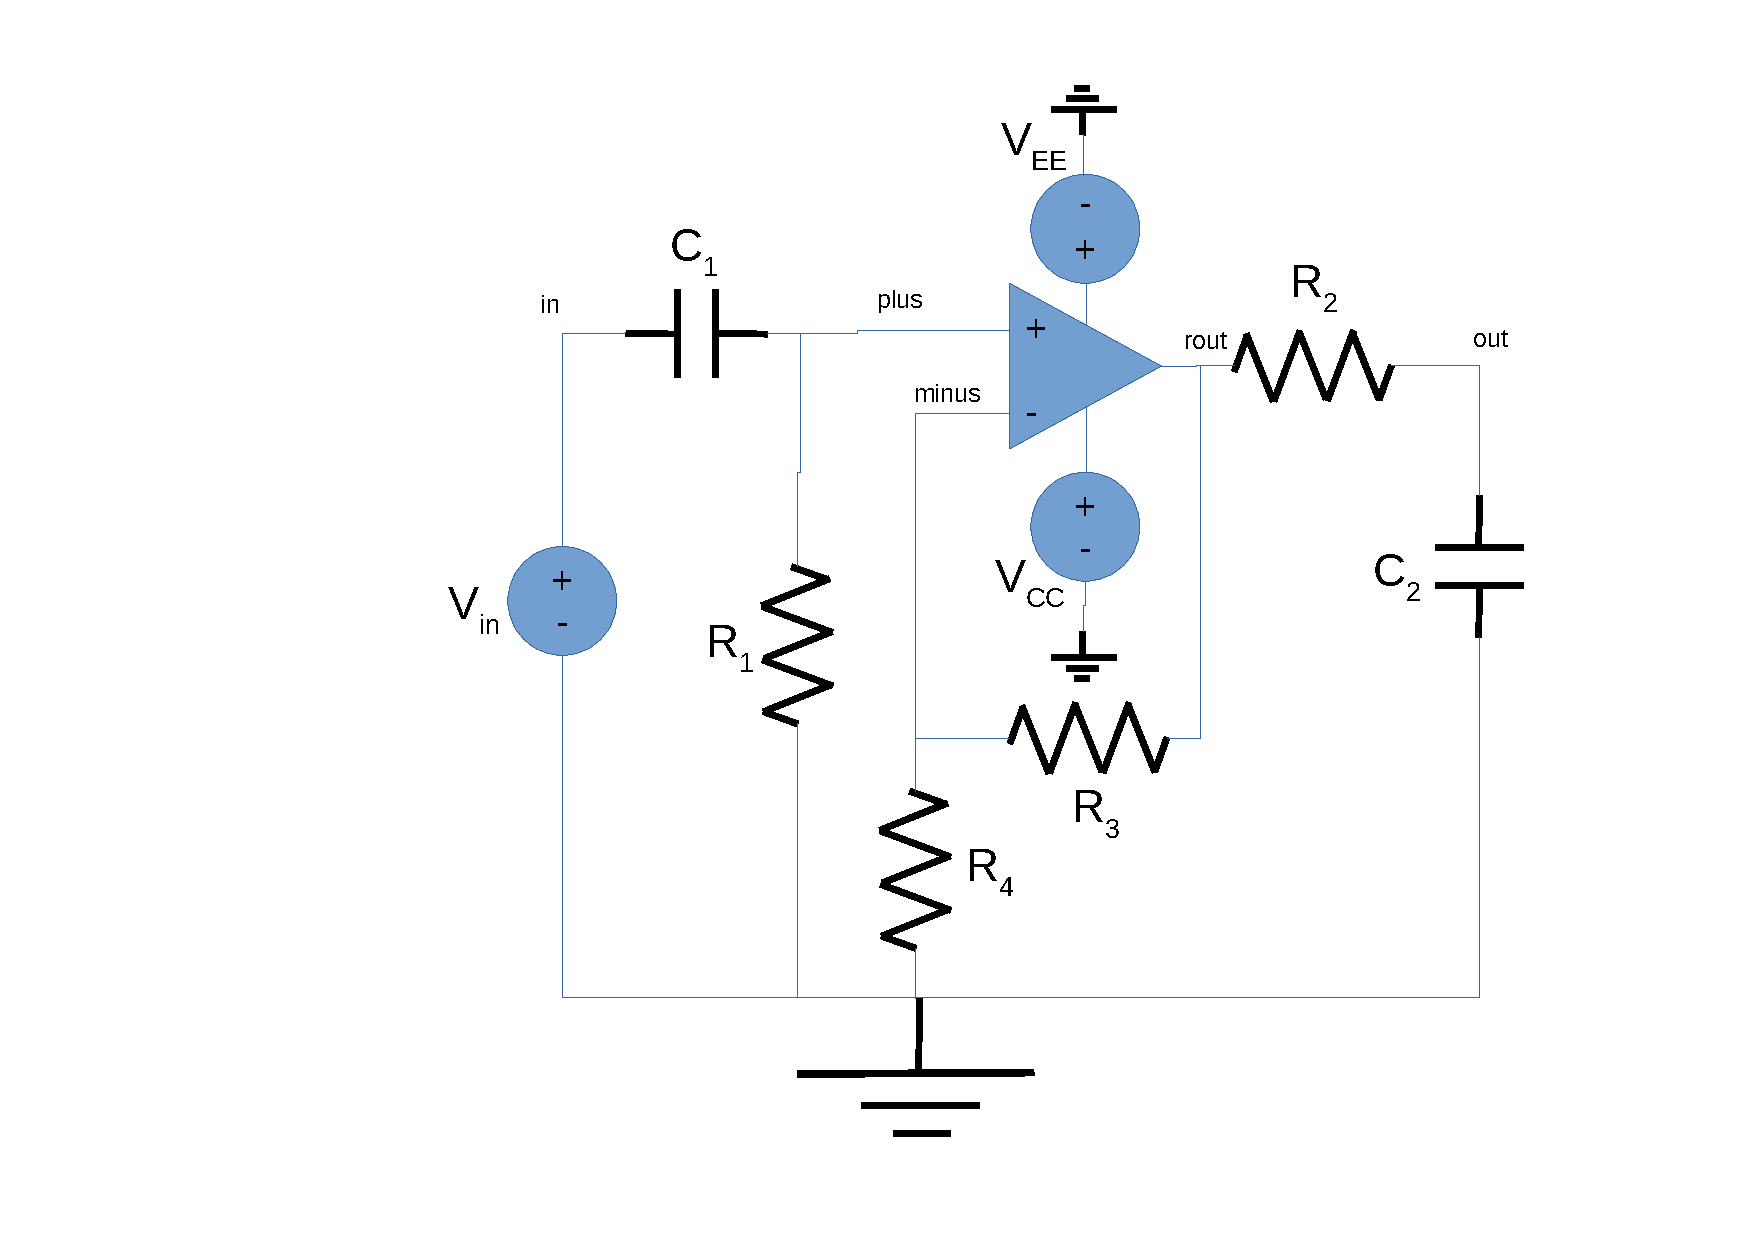
\includegraphics[width=0.6\linewidth]{circuit.pdf}
\caption{The circuit we will be working with.}
\label{fig:circuit}
\end{figure}


Firstly, in Section~\ref{sec:simulation}, the circuit is analysed by simulating it as a whole, using the \textit{software Ngspice}.

After that, we proceed to the theoretical analysis of this same circuit to verify and compare results with the simulation data. In Section ~\ref{sec:analysis}, the theoretical analysis is executed in two distinct steps: the first step consists of a operating point analysis, where it's only considered the DC component of the current; the second step, called incremental analysis, takes into account the frequencies of the current in time, therefore, the AC component of the current.

Lastly, in Section \ref{sec:comparing} the results obtained in the two previous Sections are compared, focusing on the currents and tensions obtained in key points of the circuit. as well as, impedances and gain.
The conclusions of this study are outlined in Section~\ref{sec:conclusion}.